\documentclass[10pt]{article}
\usepackage[T1]{fontenc}
\usepackage[english]{babel}
\usepackage[utf8]{inputenc}
\usepackage{fullpage}
\usepackage{url}
\usepackage{varioref}
\usepackage{braket}
\usepackage{graphicx}
\usepackage{multicol}
\usepackage{amsmath,amssymb}
\usepackage{mathtools}	

\def\te{{\rm e}}

\title{One-dimensional chain of identical harmonic oscillators}
\author{Kristian Knakkergaard Nielsen}
\begin{document}
\maketitle

\section{System: in real space and in momentum space}
We consider a one dimensional chain of $N$ identical harmonic oscillators to model a 1D solid. We will impose cyclic boundary conditions as to avoid boundary effects. Classically this means that we have a circular chain of masses $m$ connected by perfect Hooke springs. Quantum mechanically we will think of these masses as the atoms in the solid. The harmonic oscillator description is the lowest order description of the system. Can you guess why? Argue hereby that the Hamiltonian of the system is
\begin{equation}
H = \sum_{j=1}^N \left(\frac{p_j^2}{2m} + \frac{1}{2}m\Omega^2(x_j-x_{j+1})^2 \right)
\label{eq.hamiltonian_real_space}
\end{equation}

Here $p_j$ is the momentum operator for the $j$'th atom, and $x_j$ is the \textit{displacement} operator from equilibrium distance $a$ between the masses. The cyclic boundary conditions means that $x_{j+N}=x_j$, (why?!). We would like to figure out the dispersion relation $\omega(k)$ connecting the frequency of oscillation to the crystal momentum $k$. We will elaborate on the term 'crystal momentum' later on. Hence, we would like to operate in momentum space. In this procedure we also hope to uncouple the coupled harmonic oscillators in $j$ and $j+1$. To do this we shall later see that it is nice to express the operators $x_j$ and $p_j$ in terms of new operators $x_k$ and $p_k$
\begin{equation}
x_j = \frac{1}{\sqrt{N}}\sum_k x_k \te^{ikja}, \; \;  p_j = \frac{1}{\sqrt{N}}\sum_k p_k\te^{ikja}. 
\label{eq.fourier_decomp_xjpj}
\end{equation}
This is an implicit definition of the new operators. We will now figure out what we are actually summing over and find an explicit expression for $x_k, p_k$. First show that because of the cyclic boundary conditions, $x_{j + N} = x_j, p_{j + N} = p_j$, then $\exp(ikNa) = 1$ and hereby that
\begin{equation}
k = n\frac{2\pi}{Na}, \nonumber
\end{equation}
where $n$ is an integer. Hence the boundary condition leads to a specific \textit{quantization} of allowed $k$'s. We still don't know how many $k$'s there are though. Now show that
\begin{equation}
\frac{1}{\sqrt{N}}\sum_{j = 1}^{N} \te^{-ikja} x_j = \sum_{k'} \left[\frac{1}{N}\sum_{j = 1}^{N} \te^{i(k' - k)ja}\right]x_{k'}. \nonumber
\end{equation}
and likewise for the $p$-operators. Now read the wikipedia page on the \textit{geometric sum}. Use it to show that
\begin{equation}
\frac{1}{N}\sum_{j = 1}^{N} \te^{i(k'-k)ja} = \delta_{k', k}. \nonumber
\end{equation}
You have thus shown that
\begin{equation}
x_k = \frac{1}{\sqrt{N}}\sum_{j=1}^N x_j\te^{-ikja}, \; \; p_k = \frac{1}{\sqrt{N}}\sum_{j=1}^N p_j\te^{-ikja}. 
\label{eq.fourier_decomp_xkpk}
\end{equation}
Further show that $p_k^\dagger = p_{-k}, x_k^\dagger = x_{-k}$. Hence the operators $p_k$ and $x_k$ are \textit{not} hermitian! Now show that $p_{k+2\pi m/a}=p_k$ and likewise for $x_k$. This tells us that $k$'s equal up to a multiple of $\frac{2\pi}{a}$ are equivalent, and so we can restrict ourselves to $k\in (-\pi/a, \pi/a]$.  This is the so-called Brillouin zone! Hence we only have to consider these momenta
\begin{equation}
k_n = n\frac{2\pi}{Na}, \; \; n = -\frac{N}{2}+1, -\frac{N}{2}+2, \dots, \frac{N}{2}. 
\end{equation}
Notice that in total, there are $N$ momenta! By using that $[x_j,p_{j'}]=i\hbar \delta_{j,j'}$, show that
\begin{equation}
[x_k,p_{k'}]=i\hbar \delta_{k,-k'}. 
\end{equation}

Now insert \eqref{eq.fourier_decomp_xjpj} into equation \eqref{eq.hamiltonian_real_space} and show that
\begin{equation}
H = \sum_k \left(\frac{p_{-k}p_k}{2m}+2m\Omega^2\sin^2\left(\frac{ka}{2}\right) x_{-k}x_k\right)
\label{eq.hamiltonian_momentum_space}
\end{equation}

The Hamiltonian is hereby uncoupled in $k$ (since $p_{-k}=p_k^\dagger$, likewise for $x_k$). Argue that this defines harmonic oscillators with mass $m$ and angular frequencies
\begin{equation}
\omega(k)= 2\Omega\left|\sin\left(\frac{ka}{2}\right)\right|. 
\end{equation}
This is the desired dispersion relation! We will come back to this! 
(Hint: for each $k$ compare the $k$'th term in the sum in equation \eqref{eq.hamiltonian_momentum_space} with the normal expression for a single harmonic oscillator $H = \frac{p^2}{2m}+\frac{1}{2}m\omega^2 x^2$). 

\section{'a' operators, ground state and excited states}
By looking at the 'algebraic method' in Griffith's argue that for each $k \neq  0$ we should define
\begin{equation}
a_k = \left(\frac{m\omega(k)}{2\hbar}\right)^{1/2}\left(x_k+\frac{i}{m\omega(k)}p_k \right). 
\label{eq.a_operator}
\end{equation}
What is the problem for $k=0$? Show that
\begin{equation}
a_k^\dagger= \left(\frac{m\omega(k)}{2\hbar}\right)^{1/2}\left(x_{-k}-\frac{i}{m\omega(k)}p_{-k} \right), 
\end{equation}
and that $[a_{k'},a_k^\dagger]=\delta_{k',k}$, with all other commutators 0. This is quite crucial, and we will return to it later on. Now either argue or show explicitly that
\begin{equation}
H = \frac{p_{k=0}^2}{2m}+\sum_{k\neq 0}\hbar \omega(k)\left(a_k^\dagger a_k+\frac{1}{2}\right), \; \;  \omega(k)= 2\Omega\left|\sin\left(\frac{ka}{2}\right)\right|
\end{equation}

This looks a little different than the usual case of one harmonic oscillator. Firstly, there is a sum over all $k\neq 0$. Secondly, the $k=0$ term is special because we cannot make the transformation to the 'a' operators (why?!). Now let $\hat{P}=\sum_j p_j$ be the total momentum of the solid, and show that $p_{k=0} = \frac{\hat{P}}{\sqrt{N}}$. This means that we can write the Hamiltonian as two commuting terms
\begin{align}
H &= \frac{1}{N}\frac{\hat{P}^2}{2m} + \sum_{k\neq 0}\hbar \omega(k)\left(a_k^\dagger a_k+\frac{1}{2}\right) \\
    &= \frac{1}{N}\frac{\hat{P}^2}{2m} + H_{\text{ph}}.
\label{eq.hamiltonian_a_operators}
\end{align}

Argue that this means that the states can be written as product states of eigenstates to $\hat{P}$ and $H_{\text{ph}}$. The subscribt `ph' refers to \textit{phonons} as we shall elaborate on later. Further argue that the ground state $\ket{0}$, has $\hat{P}\ket{0} = 0$ and $a_k\ket{0}=0$ for all $k\neq 0$. Show that the energy $E_0$ of the ground state hereby is
\begin{equation}
E_0 = \frac{1}{2}\sum_k\hbar\omega(k) = \frac{2}{\pi}N\hbar\Omega,
\end{equation}
where the last equality is only for $N\gg 1$. (Hint: apply $H$ to $\ket{0}$. Then change the sum into an integral and solve it). This means that the energy per atom is $E_0/N = 2/\pi \hbar\Omega$ in the ground state. Now imagine that we instead had a collection of $N$ separate particles all connected to 2 springs. Argue that the energy per particle is $\hbar \Omega$. Why is the energy per particle ($E_0/N$) in the solid lower than for the separate particles? 

The eigenstates to $H_{\text{ph}}$ can now be formed by using $a_k^\dagger$ operators on the ground state $\ket{0}$. Argue that these states, properly normalized, are of the form
\begin{equation}
\ket{l_1, l_2, \dots, l_N} = \frac{1}{\sqrt{l_1!}}(a_{n=-\frac{N}{2}+1}^\dagger)^{l_1}\frac{1}{\sqrt{l_2!}}(a_{n=-\frac{N}{2}+2}^\dagger)^{l_2}\cdots \frac{1}{\sqrt{l_N!}}(a_{n=\frac{N}{2}}^\dagger)^{l_N}\ket{0}. 
\end{equation}

For brevity we have writen $a^\dagger_n$ in stead of $a^\dagger_{k_n}$. Hence, $a^\dagger_n$ is understood as the creation operator belonging to $k_n = \frac{n 2\pi}{Na}$. Further show that the energy of such a state is
\begin{equation}
E(\ket{l_1, l_2, \dots, l_N}) = \sum_{j=1}^{N}\hbar\omega(k_j)\left(l_j+\frac{1}{2}\right)
\end{equation}

We say that the state has $l_j$ quanta or \textit{phonons} in the $j$'th oscillator. The term phonon hereby refers to an excited state of $H_\text{ph}$ (ph is short for phonon). We shall see that they actually signify oscillatory states in the solid, and the number of phonons tells us how many such oscillatory states there are. In this context $a_k$ ($a_k^\dagger$) is said to annihilate (create) a phonon of crystal momentum $\hbar k$. 

In the following two sections we will investigate the oscillatory states. Here we will also use a slightly different notation for the states: $\ket{1_k} = a^\dagger_k \ket{0}$. Hence the number, here 1, refers to the number of phonons in the state. The subscript $k$ refers to the crystal momentum of the phonon.  

\section{Physical significance of dispersion relation}
Start by reading the wiki-page: \url{https://en.wikipedia.org/wiki/Dispersion_relation}. Now show that
\begin{equation}
\left.\frac{\partial \omega}{\partial k}\right|_{k=0^+} = \Omega a, 
\end{equation}
and hereby that $\omega(k) =  \Omega ak$ for small $k>0$. Hence the group velocity $\frac{\partial \omega}{\partial k}$ and the phase velocity $\omega/k$ are the same for small $k$. Argue hereby that for small $k$ the solid propagates sound with the speed of sound $v=\Omega a$!

\section{Phonons are bosons}
As you might have learned by now all particles are sorted into fermions and bosons, depending whether they have half-integer or integer spin. As described by Griffith in your quantum mechanics book, bosons have symmetric whilst fermions have antisymmetric wave functions. The commutator relation $[a_k,a_{k'}^\dagger]=\delta_{k,k'}$ actually tells us what kind of 'particle' (we call it a quasiparticle, because it is not a fundamental particle) a phonon is. Say we have a state with one phonon of momentum $k$ and one phonon with momentum $k'$. Then the state is
\begin{equation}
\ket{1_k,1_{k'}} = a_k^\dagger a_{k'}^\dagger\ket{0} = \frac{1}{2}(a_k^\dagger a_{k'}^\dagger+a_k^\dagger a_{k'}^\dagger)\ket{0} = \frac{1}{2}(a_k^\dagger a_{k'}^\dagger+a_{k'}^\dagger a_{k}^\dagger)\ket{0} = \ket{1_{k'},1_k},
\end{equation}

since $a_k^\dagger$ and $a_{k'}^\dagger$ commute. In more general terms a bosonic state is symmetric with respect to the variables in question. Here it is the momenta $k$ and $k'$, and so we see that phonons are bosons! What do you think the spin is? \\

Further we see that the phonons are actually excitations in a harmonic oscillator for each $k$. This is of great importance for the thermodynamics of the system, as we shall see later. 

\section{Time evolution and oscillation}
In this section I will introduce a concept that is probably new for you. In your quantum mechanics course observables, like $x$ and $p$, do not evolve in time. Further physical states, the wave function, does evolve in time according to Schrödinger's differential equation $H\psi = i\hbar \frac{\partial \psi}{\partial t}$. This way to address quantum mechanics is called the Schrödinger picture. \\

In this section we will switch to the Heisenberg picture of quantum mechanics. Here it is the observables, like $x$ and $p$, that evolve in time, while the states remain constant in time. For a deeper discussion of this I encourage you to read in \cite{Sakurai} pp.  80-86. I can give you a copy of those pages, if you would like them. There Heisenberg's equation of motion is also derived. Actually you just have to take Ehrenfest's theorem and neglect the averaging. Explicitly for an operator $A$ in the Heisenberg picture:
 \begin{equation}
 \frac{d A}{dt} = \frac{1}{i\hbar}[A,H]. 
 \end{equation}
 
 And so the commutator determines the time evolution of the operator. Here we are interested in first to calculate the time evolution of our creation and annihilation operators $a_k^\dagger, a_k$. Show, using equation \eqref{eq.hamiltonian_a_operators} that for $k\neq 0$
 \begin{equation}
 \frac{d a_k}{dt} = \frac{1}{i\hbar}[a_k,H] = -i\omega(k)a_k.  
 \end{equation}
 
 Therefore: $a_k(t) = a_k(0)\te^{-i\omega(k)t}$. We will simply, but perhaps a little confusingly, write $a_k(0)=a_k$. This further means that $a_k^\dagger(t)=a_k^\dagger \te^{i\omega(k)t}$. Now we are ready to study oscillations in our system. From equation \eqref{eq.a_operator} show that
 \begin{equation}
 x_k(t) = \frac{1}{2}\left(\frac{2\hbar}{m\omega(k)}\right)^{1/2}\left(a_k\te^{-i\omega(k)t} + a_{-k}^\dagger\te^{i\omega(k)t}\right). 
 \end{equation}
 
Hereby we can also express $x_j(t)$ using the creation and annihilation operators. Argue that for purely oscillatory states $x_j(t)$ is
\begin{equation}
x_j(t)=\left(\frac{\hbar}{mN}\right)^{1/2}\sum_{k\neq 0}\frac{1}{\sqrt{2\omega(k)}}\left( a_k\exp\left[i(kja-\omega(k)t)\right]+a_{-k}^\dagger\exp\left[-i(-kja-\omega(-k)t)\right] \right).
 \label{eq.x_field_expansion}
 \end{equation}
 
This is a field expansion of the particle position. Notice that the position operator is an expansion in creation and annihilation operators and corresponding plane waves with momenta $k$ and $-k$ at positions $ja$ and energy $\hbar\omega(k)$. Now classically we expect oscillatory modes in the chain. To investigate this quantum mechanically we look at the single phonon eigenstates $\ket{1_k}=a_k^\dagger\ket{0}$ for $k\neq 0$. Show that $\bra{1_k}x_j(t)\ket{1_k} = \bra{0}a_kx_j(t)a_k^\dagger\ket{0}=0$. Why is this not surprising?
To quantify the motion of the atoms we will look at the covariance of the position of the $j$'th atom at time $t$ to the position of the $l$'th atom at time $t=0$ in the $k$'th oscillatory mode 
\begin{equation}
\text{Cov}_k(x_j(t),x_l(0)) = \bra{1_k} x_j(t)x_l(0)\ket{1_k} - \bra{1_k} x_j(t)\ket{1_k}\bra{1_k} x_l(0)\ket{1_k} =  \bra{1_k} x_j(t)x_l(0)\ket{1_k}. 
\end{equation}

The reason for this is that a positive covariance shows a tendency of the variables to have corresponding high values, whilst a negative covariance shows a tendency of high values of one to correspond to low values of the other. Argue now, why this means that $\bra{1_k} x_j(t)x_l(0)\ket{1_k}$ is a measure of how the $j$'th atom oscillates relative to the $l$'th atom. Further show that
\begin{align}
\bra{1_k} x_j(t)x_l(0)\ket{1_k} &= \bra{0} x_j(t)x_l(0)\ket{0} + \frac{\hbar}{Nm\omega(k)}\cos\left(k(j-l)a-\omega(k)t\right) \\
&=  \bra{0} x_j(t)x_l(0)\ket{0} + \frac{\hbar}{Nm\omega(k)}\cos\left(k\left(ja-\frac{\omega(k)}{k}t\right)-kla\right),
\end{align}

for all $k\neq 0$. Since $ja$ is the equilibrium position of the $j$'th atom, argue that the second part in the above expression describes a wave traveling through the solid without distortion. What is the speed of the wave? How about for small $k$? When is the speed of the wave the highest? When are the oscillations the largest? We now look at the underlying oscillations in the ground state through $\bra{0} x_j(t)x_l(0)\ket{0}$. Show that
\begin{equation}
\bra{0} x_j(t)x_l(0)\ket{0} = \frac{\hbar}{2Nm}\sum_{q \neq 0} \frac{1}{\omega(q)}\te^{-i\omega(q)t}\cos(q(j-l)a).
\label{eq.ground_state_osc}
\end{equation}

This shows that there are significant oscillations in the ground state $\ket{0}$. By calculating $\bra{1_k}x_j^2\ket{1_k}$ and $\bra{0}x_j^2\ket{0}$ we can actually see that the oscillations in the solid are large underlying ground state oscillations with small excited state oscillations. Show explicitly
\begin{equation}
\bra{1_k}x_j^2(t)\ket{1_k} = \bra{0}x_j^2(t)\ket{0} + \frac{\hbar}{mN}\frac{1}{\omega(k)}, \; \;  \bra{0}x_j^2(t)\ket{0} = \frac{\hbar}{2mN}\sum_{q\neq 0} \frac{1}{\omega(q)}. 
\end{equation}

Now try making a plot of $\text{Re}\left[\bra{0} x_j(t)x_1(0)\ket{0}\right]$ for $N = 50$ and all $j$. It should look something like figure \ref{fig.ground_state_osc}. From here argue that there is a wave traveling from $x=a$ through the solid with a group speed of $v=\Omega a$, which is slowly being distorted. Why is it traveling with $v=\Omega a$, and why is it getting distorted? What we are investigating can be formulated in the following way (if you don't agree, we can discuss this!): when we investigate how the atoms oscillate relative to the first atom in the chain in the ground state, we excite a localized wave at the first atom that travels through the solid. This is what can be observed in the figure. Hence by measuring on the solid we are disturbing it! 

\begin{figure}
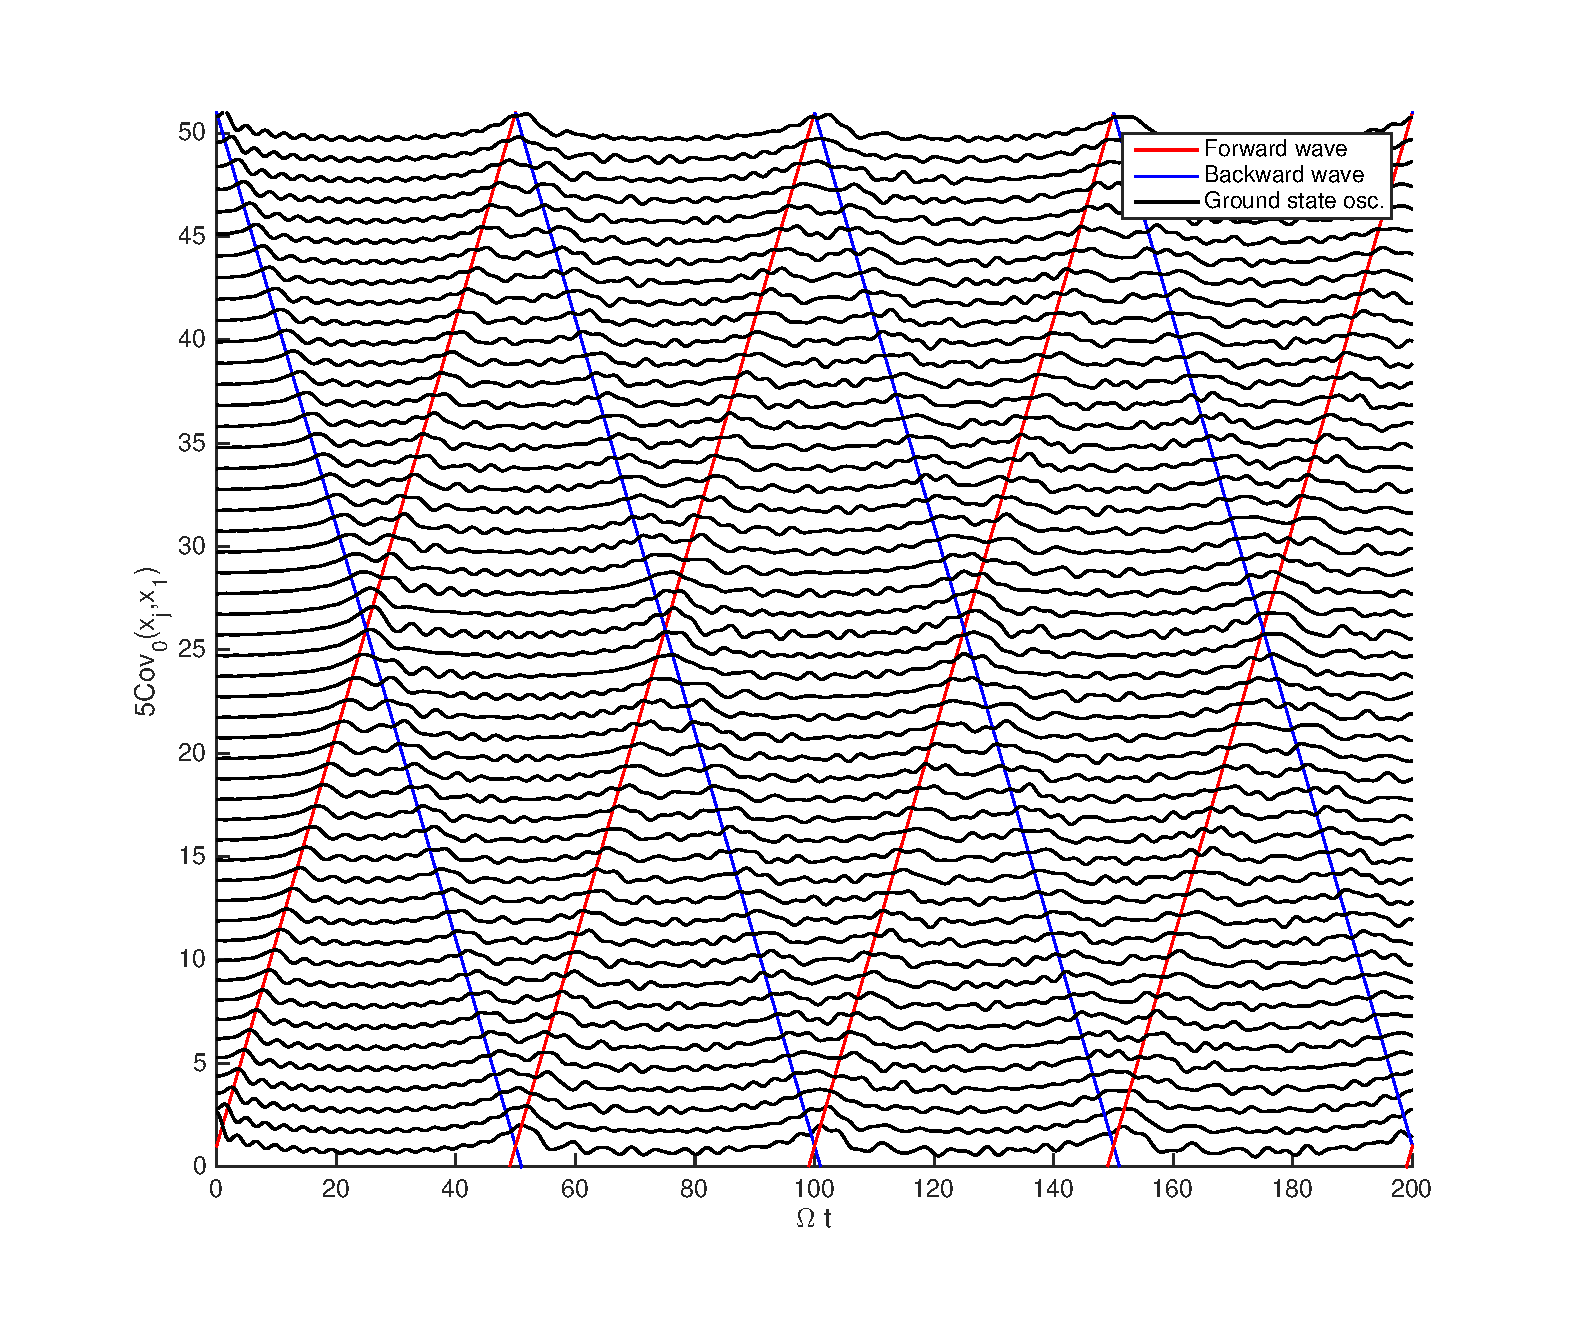
\includegraphics[width=1\textwidth]{ground_state_osc.eps} 
\caption{\textsl{The ground state oscillations $\text{Cov}_0(x_j(t),x_1(0))=\bra{0} x_j(t)x_1(0)\ket{0}$ are plotted versus $\Omega t$ for $N = 50$. The oscillations are exaggerated by a factor of 5 to make the oscillations more visible. The $j$'th atom is shifted with its equilibrium position $ja$. I have set $a=1$. The red (blue) line shows that there is a forward (backward) traveling wave, traveling with the speed $v=\Omega a$. Notice that the wave is distorted more and more. }}
\label{fig.ground_state_osc} 
\end{figure} 

%\begin{figure}
%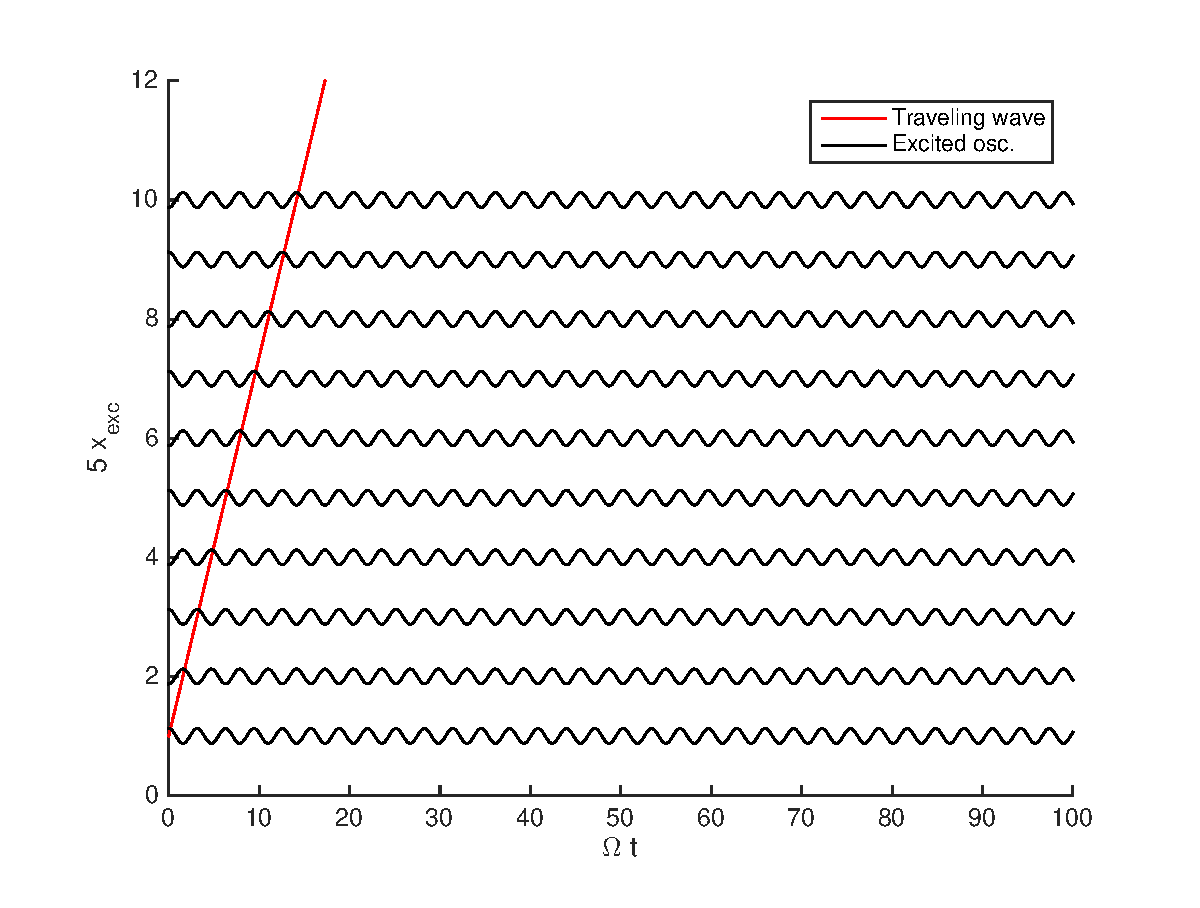
\includegraphics[width=1\textwidth]{exc_osc.eps} 
%\caption{\textsl{The excited state oscillations for $k=\pi/a$ are plotted versus $\Omega t$ for $N=10$. Here the underlying ground state oscillations have been neglected. The $j$'th atom is shifted with its equilibrium position $ja$.  The red line shows the propagation of a wave with the speed $\omega(k)/k$. }}
%\label{fig.exc_osc} 
%\end{figure} 

%%%%%%%%%%%%%%%%%%%%
\section{Controlled disturbance}
In the previous section we saw some uncontrolled oscillations in the solid. Here we will see how the solid reacts to a (controlled) displacement of a number of the atoms. First show that

\begin{equation}
x_j(t) = \frac{1}{\sqrt{N}}\sum_{k\neq 0} \te^{ikja}\left[x_k\cos(\omega(k)t)+\frac{p_k}{m\omega(k)}\sin(\omega(k)t) \right]. 
\label{eq.xj_xk_pk}
\end{equation}
This is comparable to equation (2.3.45a) in \cite{Sakurai}. 
Now argue that $\ket{\alpha}=\exp\left(-\frac{i}{\hbar}\sum_l p_l b_l\right)\ket{0}$ is a state, where we have displaced the $l$'th atom a distance $b_l$ at $t=0$. We would now like to calculate the mean value of $x_j(t)$: $\bra{\alpha}x_j(t)\ket{\alpha}$. (Hint: this is a little tricky. Read pp. 41-50 in \cite{Sakurai}). By using $p_l = \frac{1}{\sqrt{N}}\sum_q p_q\exp(iqla)$, show that
\begin{equation}
\bra{\alpha}x_j(t)\ket{\alpha} = \frac{1}{\sqrt{N}}\sum_{k\neq 0}e^{ikja}\cos(\omega(k)t)\bra{0}\exp\left(\frac{i}{\hbar \sqrt{N}}p_{-k}\sum_l e^{-ikla}b_l\right)x_k\exp\left(-\frac{i}{\hbar \sqrt{N}}p_{-k}\sum_l e^{-ikla}b_l\right)\ket{0}. \nonumber
\end{equation}
Now first show that: $\left[x_k, p_{-k}^n\right] = i\hbar np_{-k}^{n-1}$ for positive integers $n$. Then show that for a function of $p_{-k}$, $f(p_{-k})$, which has a Taylor expansion
\begin{equation}
\left[x_k, f(p_{-k})\right] = i\hbar \frac{\partial f}{\partial p_{-k}}.
\end{equation}
Hint: write $f(p_{-k}) = \sum_{n = 0}^{\infty} \frac{f^{(n)}(0)}{n!}p_{-k}^n$. Then use the commutator of $x_k$ and $p_{-k}^n$ in each term! Use this to show that
\begin{equation}
\left[x_k, \exp\left(-\frac{i}{\hbar \sqrt{N}}p_{-k}\sum_l e^{-ikla}b_l\right) \right] = \frac{1}{\sqrt{N}}\sum_l b_l e^{-ikla}\exp\left(-\frac{i}{\hbar \sqrt{N}}p_{-k}\sum_l e^{-ikla}b_l\right). \nonumber
\end{equation}
Use this to show
\begin{equation}
\bra{\alpha}x_j(t)\ket{\alpha} = \frac{1}{N}\sum_{k\neq 0} e^{ikja}\cos(\omega(k)t)\sum_l b_l e^{-ikla} = \frac{2}{N}\sum_{k>0} \cos(\omega(k)t)\sum_l b_l\cos(k(j-l)a).
\label{eq.mean_value_controlled_osc}
\end{equation}
This was for a general displace $b_l$. We see explicitly that it is real (as it should be!!). Now let us take a simple example: $b_l = (-1)^l b$, for some positive displacement $b$. Show
\begin{equation}
\sum_l b_l e^{-ikla} = b\sum_l e^{-i(ka-\pi)l} = Nb\delta_{k,\pi/a}.\nonumber
\end{equation}
(Hint: $e^{i\pi} = -1$). Hence for this specific set of initial values, we get
\begin{equation}
\bra{\alpha}x_j(t)\ket{\alpha} = b e^{ij\pi}\cos\left(\omega\left(\frac{\pi}{a}\right)t\right) = (-1)^j b\cos\left(\omega\left(\frac{\pi}{a}\right)t\right). 
\end{equation}
Characterize this oscillation classically. We can also let $b_l=b$ for $l=1$ and $0$ otherwise. Then
\begin{equation}
\bra{\alpha}x_j(t)\ket{\alpha} = \frac{2b}{N}\sum_{k>0} \cos(\omega(k)t) \cos(k(j-1)a).
\end{equation}
Notice the similarity with equation \eqref{eq.ground_state_osc}. Make a plot of this similar to figure \ref{fig.ground_state_osc}, and identify a traveling wave. Argue by going through your calculation that it makes no difference to the result, if we let  $\ket{\alpha}=\exp\left(-\frac{ip_l b}{\hbar}\right) a_k^\dagger \ket{0}$ for some $k\neq 0$ instead. Hence, the disturbance travels in the same manner in the excited states. 

%%%%%%%%%%%%%%%%%%%%
\section{The $k=0$ mode}
Now we have investigated the oscillations of the solid. By remembering the Hamiltonian as written in equation \eqref{eq.hamiltonian_a_operators}, we know that we have total momentum eigenstates of the solid coming from the $k=0$ term in the Hamiltonian. For this reason it is often referred to as the $k=0$ mode. Please notice that $P$ can have any value, and that this shows that we cannot interpret the $\hbar k$'s as pure momentum, since $k=0$ here! In spite of this phonons for $k\neq 0$ takes part in scattering events with e.g. electrons in solids as if they had momentum $\hbar k$. For this reason $\hbar k$ is often referred to as crystal momentum. 


\newpage
\section{Thermodynamics of the system}
This section is concerned with the thermodynamic limit $N\gg 1$. As we now have seen phonons are bosons and excitations in a harmonic oscillator. They therefore obey the Planck distribution for each $k$, and for each $k$ we have energies: $0, \hbar\omega(k), 2\hbar\omega(k), \dots$ relative to the ground state. Now we wish to calculate the so-called partition function using Boltzmann statistics. It is defined and discussed in \cite{Schroeder} pp. 220-231
\begin{equation}
Z_k = \sum_{n=0}^\infty \exp(-\beta n\hbar\omega(k)) =  \sum_{n=0}^\infty (\exp(-\beta \hbar\omega(k)))^n,
\end{equation}
where $\beta = \frac{1}{k_BT}$, and $T$ is the temperature. Show that $Z_k = \frac{1}{1-\exp(-\beta\hbar\omega(k))}$. (Hint: geometric sum).  Further the \textit{mean energy} $U_k$ for each $k$ can, according to exercise 6.16 in \cite{Schroeder}, be calculated as $U_k = -\frac{1}{Z_k}\frac{\partial Z_k}{\partial \beta}$. By using this, show that

\begin{equation}
U_k = \frac{\hbar\omega(k)}{\exp(\beta\hbar\omega(k))-1}
\end{equation}
Hereby the total mean energy is $U=\sum_k U_k$. Now remember that $k=n\frac{2\pi}{Na}$, and so the difference between neighbouring $k$'s are $\Delta k = \frac{2\pi}{Na}$. Hereby show that

\begin{equation}
U = \frac{Na}{2\pi}\sum_k\frac{\hbar\omega(k)}{\exp(\beta\hbar\omega(k))-1}\Delta k 
\end{equation}
In the thermodynamic limit $N\gg 1$ the variation of the function $U_k$ is slow over $\Delta k$. Argue that we can hereby replace the sum with an integral

\begin{equation}
U = \frac{Na}{2\pi}\int_{-\pi/a}^{\pi/a}\frac{\hbar\omega(k)}{\exp(\beta\hbar\omega(k))-1}dk.
\end{equation}
By changing variable to $\epsilon =\hbar\omega$, show that
\begin{equation}
U = \frac{N}{\pi\hbar\Omega}\int_{0}^{2\hbar\Omega}\frac{1}{\sqrt{1-\left(\frac{\epsilon}{2\hbar\Omega}\right)^2}}\frac{\epsilon}{\exp(\beta\epsilon)-1}d\epsilon.
\end{equation}
Now read about 'density of states' pp. 279-282 in \cite{Schroeder}. Then show that the density of states here is

\begin{equation}
g(\epsilon) = \left\{\begin{matrix}
 \frac{N}{\pi \hbar\Omega}\frac{1}{\sqrt{1-\left(\frac{\epsilon}{2\hbar\Omega}\right)^2}}, & 0 \leq \epsilon < 2\hbar\Omega, \\ 
0, & \text{otherwise}.  
\end{matrix}\right. 
\end{equation}
Now let $y = \beta\epsilon$, and $\tau = \frac{1}{2\beta\hbar\Omega} = \frac{k_BT}{2\hbar\Omega}$. Consider that $y$ is the energy to temperature ratio, whilst $\tau$ is a measure of the temperature relative to the fundamental energy $2\hbar\Omega$, both without units. Show that expressed through $y$ and $\tau$ the integral for $\tilde{U}=\frac{U}{2\hbar\Omega}$ becomes

\begin{equation}
\tilde{U} = \frac{2N\tau^2}{\pi}\int_{0}^{1/\tau}\frac{1}{\sqrt{1-\left(y\tau\right)^2}}\frac{y}{\exp(y)-1}dy.
\label{eq.U_unitless}
\end{equation}
Hence, the density of states expressed through $y$ is $g(y)=\frac{2N\tau^2}{\pi}\frac{1}{\sqrt{1-\left(y\tau\right)^2}}$ for $0\leq y\tau<1$ and $0$ otherwise. Make a plot of this for some values of $\tau$ (since $N$ is just a scaling factor here you can set it to whatever you like, or simply neglect it in the plot). We have hereby expressed the energy and density of states purely in terms of unitless quantities. Now we want to compute the energy in two limits. First we take the low temperature limit: $k_BT\ll 2\hbar\Omega$ or in other words $\tau \ll 1$. Argue that a very good approximation for  $\tilde{U}$ is now

\begin{equation}
\tilde{U} = \frac{2N\tau^2}{\pi}\int_{0}^{\infty}\frac{y}{\exp(y)-1}dy.
\end{equation}
Evaluate the integral to get $\tilde{U} = \frac{\pi N\tau^2}{3}$ (it is okay to use Maple, Mathematica or stuff like that, it is a tricky integral). Equivalently we have

\begin{equation}
U = \frac{\pi N}{6\hbar\Omega}(k_BT)^2. 
\end{equation}
Hence the total mean energy goes quadratically to $0$. Calculate the heat capacity at constant volume $C_V = \frac{\partial U}{\partial T}$ (with all other variables held constant). Comment on the result with respect to freezing out degrees of freedom and in relation to the so-called third law of thermodynamics discussed in \cite{Schroeder} pp. 93-95. In the opposite (high temperature) limit, so that $\tau \gg 1$, show that

\begin{equation}
U = Nk_BT.
\end{equation}
Hint: take \eqref{eq.U_unitless} and argue that it is a good approximation to make the expansion $\exp(y) = 1+y$. Then evaluate the resulting integral. If you need help, just ask ;).  Comment on the result, and how we could have stated this without any calculations using the equipartition theorem (the theorem is \textit{derived} in \cite{Schroeder}, but you also saw it in your 'Mekanik \& Termodynamik' course). Calculate the heat capacity. If you are able to do so, make a numerical calculation of $U$ for all values of $\tau$ and plot it together with the asymptotic forms derived here! \\


\newpage
\begin{thebibliography}{99}
\bibitem{Sakurai} Modern Quantum Mechanics, Revised edition, J.J. Sakurai,  1994
\bibitem{Schroeder} An Introduction To Thermal Physics, Weber State University, Daniel V. Schroeder, 2000
\end{thebibliography}

\end{document}
